\documentclass[]{article}
\usepackage[T1]{fontenc}
\usepackage[acronym, toc]{glossaries}
\usepackage{graphicx}
\usepackage{float}
\usepackage{amsmath}
\usepackage{amsfonts}
\usepackage{amssymb}

\graphicspath{{./charts/}}

%opening
\title{{{\normalsize Sprawozdanie trzecie} \\
		{\huge Algorytmy grafowe}}}
\author{Piotr Tylczyński}
\date{20.04.2019}


\newglossaryentry{n}{
	name={n},
	description={ilość wierzchołków w grafie}
}

\newglossaryentry{m}{
	name={m},
	description={ilość krawędzi w grafie}
}

\newglossaryentry{G}{
	name={G},
	description={skierowany graf acykliczny, w którym wierzchołki są etykietowane kolejnymi liczbami naturalnymi zaczynając od 0}
}

\newglossaryentry{A}{
	name={A},
	description={dowolny wierzchołek w \gls{G}, różny od \gls{B}}
}

\newglossaryentry{B}{
	name={B},
	description={dowolny wierzchołek w \gls{G}, różny od \gls{A}}
}
\makeglossaries


\begin{document}

\renewcommand*\contentsname{Spis}
\maketitle
\tableofcontents
\clearpage

\section{Reprezentacja grafu przez macierz sąsiedztwa}
	\subsection{Opis}
		W tej reprezentacji \gls{G} jest opisywany przez zero-jedynkową macierz o \gls{n} kolumnach i \gls{n} wierszach. W \gls{G} istnieje łuk między wierzchołkami \gls{A} i \gls{B}, jeżeli istnieje jedynka w macierzy sąsiedztwa znajdująca się w \gls{A} kolumnie i \gls{B} wierszu.
	\subsection{Złożonośc podstawowych operacji}
		\subsubsection{Sprawdzenie istnienia krawędzi}
			Posiada złożoność:
			\begin{equation}
				O(1)
			\end{equation}
			Złozonośc jest stała, ponieważ sprawdzenie istnienia krawędzi sprowadza się do sprawdzenia, czy w odpowiednim miejscu macierzy znajduje się jedynka. Odczytanie pola elementu z tabeli posiada stałą złożoność czasową, więc i operacja sprawdzania istnienia krawędzi jest stała
		\subsubsection{Znalezienie wszystkich nastepników}
			Posiada złożność
			\begin{equation}
				O(n)
			\end{equation}
			Znalezienie nastepników w macierzy sąsiedztwa sprowadza sie od przejrzenia odpowiedniej kolumny w macierzy sąsiedztwa. Jak wiadomo macierz sąsiedztwa posiada dokładnie \gls{n} elementów w kolumnie, a złożoność odczytania jednego elementu jest stała, więc odczytanie $n$ elementów zajmie \gls{n} czasu.
	\subsection{Sortowanie topologiczne}
		\begin{figure}[H]
			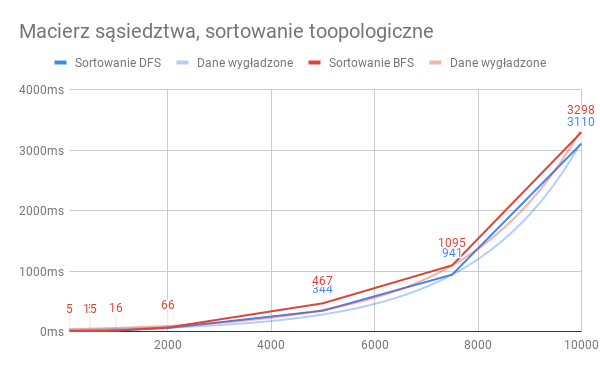
\includegraphics[scale=0.6]{adjacency_matrix.png}
		\end{figure}
		\subsubsection{Sorotowanie za pomocą algorytmu DFS}
			Charakteryzuje się złożonością:
			\begin{multline}
				\text{ilość operacji szukania następników} * n = O(n) * n = O(n^2)
			\end{multline}
		\subsubsection{Sortowanie za pomoca algorytmu BFS}
			Cechuje się złożonością:
			\begin{multline}
				\text{ilość operacji szukania następników} * n = O(n) * n = O(n^2)
			\end{multline}
\clearpage
			
\section{Reprezentacja grafu przez listę krawędzi}
	\subsection{Opis}
		\gls{G} jest w takiej reprezentacji przechowywany jako lista par uporządkowanych. W \gls{G} istnieje łuk z \gls{A} od \gls{B} wtedy i tylko wtedy, gdy istnieje dwójka $(A, B)$, w liście krawędzi
		
	\subsection{Złożoność podstawowych operacji}
		\subsubsection{Sprawdzenie istnienia krawędzi}
			Posiada złożonośc:
			\begin{equation}
				O(m)
			\end{equation}
			Wynika ona z potrzeby przejżenia całej listy w celu sprawdzenia czy istnieje w niej odpowiednia dwójka.
		\subsection{Znalezienie wszytkich następników}
			Posiada złożoność:
			\begin{equation}
				O(m)
			\end{equation}
			Tak jak w poprzednim przypadku wynika ona z potrzeby sprawdzenia całej listy w poszukiwaniu odpowiednich dwójek.
	\subsection{Sortowanie topologiczne}
		\begin{figure}[H]
			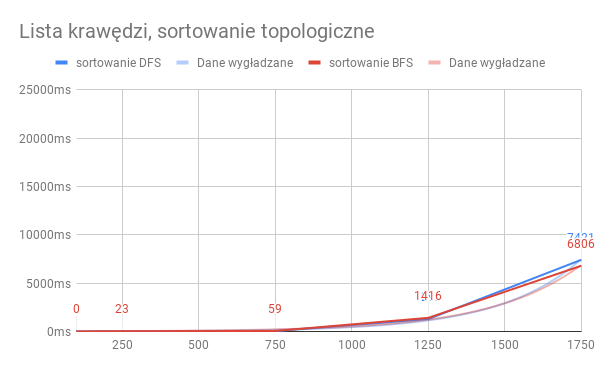
\includegraphics[scale=0.6]{edge_list.png}
		\end{figure}
		\subsubsection{Sortowanie za pomocą algorytmu DFS}
			Cechuje się złożonością
			\begin{equation}
				O(n^3)
			\end{equation}
			która wynika z:
			\begin{multline}
				\text{ilość operacji} =
				\text{ilośc operacji na poszukanie wszystkich następników} * n \\ \approx m * n 
				\label{m}
			\end{multline}
			W testownym przypdaku, czyli gdy nasycenie \gls{G} wynosi \text{50\%} ilość krawędzi można wyrazić jako:
			\begin{equation}
				m = \frac{(n)  (n - 1)}{4}
			\end{equation}
			Co po podstawieniu do równania \ref{m} daje wynik:
			\begin{equation}
				\text{ilość operacji} \approx \frac{(n)  (n - 1)}{4} *n \approx n^3 
			\end{equation}
		\subsubsection{Sortowanie za pomocą algorytmu BFS}
			Posiada złożonośc:
			\begin{equation}
				O(n^3)
			\end{equation}
			Powstała ona z:
			\begin{equation}
				\text{ilość operacji} = \text{ilość operacji na znalezienie następników} * n
			\end{equation}
			Dalszy tok rozumowania jest taki sam
\clearpage

\section{Reprezentacja grafu przez listę następników}
	\subsection{Opis}
		\gls{G} jest w takim przypadku przechowywany jako lista, której elementami są listy następników danego wierzchołka. W takim wierzchołku istnieje łuk z \gls{A} do \gls{B} jeżeli istnieje lista \gls{A}, której elementem jest \gls{B}
		
	\subsection{Złożoność podstawowych operacji}
		\subsubsection{Sprawdzanie istnienia krawędzi}
			Taka operacja ma złożoność:
			\begin{equation}
				O(n)
			\end{equation}
			co wynika z faktu, że należy przeszukać tylko jedną listę, jednak w najgorszym przypadku ta lista może składać się ze wszystkich wierzchołków \gls{G}
		
		\subsubsection{Znalezienie wszystkich następników}
			Cechuje się złożonością:
			\begin{equation}
				O(n)
			\end{equation}
			która jest spowodowana potrzebą przejrzenia odpowiedniej listy, która w najgorszym przypadku może zawierać wszystkie wierzchołki
	\subsection{Sortowanie topologiczne}
		\begin{figure}[H]
			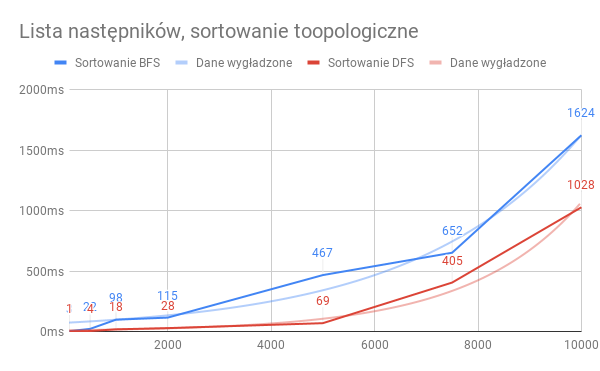
\includegraphics[scale=0.6]{adjacency_list.png}
		\end{figure}
		\subsubsection{Sortowanie za pomocą algorytmu DFS}
			Wykonuje się ze złożonością
			\begin{equation}
				O(n^2)
			\end{equation}
			powstaje one przez:
			\begin{multline}
				\text{ilośc operacji} \approx \text{ilość operacji znalezienia nastepników} * n \approx n * n \\ \approx n^2
			\end{multline}
		\subsubsection{Sortowanie za pomocą algorytmu BFS}
			Cechuje się złożonością:
			\begin{multline}
				\text{ilość operacji} \approx \text{ilość operacji szukania następników} * n \approx n * n \\ \approx n^2
			\end{multline}
		
\clearpage
\glsaddall
\printglossary[title=Zastosowane oznaczenia, toctitle=Oznaczenia]

\end{document}
